
%(BEGIN_QUESTION)
% Copyright 2011, Tony R. Kuphaldt, released under the Creative Commons Attribution License (v 1.0)
% This means you may do almost anything with this work of mine, so long as you give me proper credit

This flow control loop used to function just fine, but now it has a problem.  No matter what the setpoint value is set for on the HMI panel (touch-screen), no actual liquid flow ever goes through the pipe:

$$\includegraphics[width=15.5cm]{i02989x01.eps}$$

Identify the likelihood of each specified fault for this flow loop.  Consider each fault one at a time (i.e. no coincidental faults), determining whether or not each fault could independently account for {\it all} measurements and symptoms in this system.

% No blank lines allowed between lines of an \halign structure!
% I use comments (%) instead, so that TeX doesn't choke.

$$\vbox{\offinterlineskip
\halign{\strut
\vrule \quad\hfil # \ \hfil & 
\vrule \quad\hfil # \ \hfil & 
\vrule \quad\hfil # \ \hfil \vrule \cr
\noalign{\hrule}
%
% First row
{\bf Fault} & {\bf Possible} & {\bf Impossible} \cr
%
\noalign{\hrule}
%
% Another row
FT signal cable failed open &  &  \cr
%
\noalign{\hrule}
%
% Another row
FT signal cable failed shorted &  &  \cr
%
\noalign{\hrule}
%
% Another row
VFD signal cable failed open &  &  \cr
%
\noalign{\hrule}
%
% Another row
VFD signal cable failed shorted &  &  \cr
%
\noalign{\hrule}
%
% Another row
HMI data cable failed open &  &  \cr
%
\noalign{\hrule}
%
% Another row
PID control block in manual mode &  &  \cr
%
\noalign{\hrule}
%
% Another row
Insufficient integral control action &  &  \cr
%
\noalign{\hrule}
%
% Another row
Circuit breaker 3 tripped &  &  \cr
%
\noalign{\hrule}
%
% Another row
Circuit breaker 15 tripped &  &  \cr
%
\noalign{\hrule}
%
% Another row
Circuit breaker 22 tripped &  &  \cr
%
\noalign{\hrule}
} % End of \halign 
}$$ % End of \vbox

Finally, identify the {\it next} diagnostic test or measurement you would make on this system.  Explain how the result(s) of this next test or measurement help further identify the location and/or nature of the fault.

\underbar{file i02989}
%(END_QUESTION)





%(BEGIN_ANSWER)

% No blank lines allowed between lines of an \halign structure!
% I use comments (%) instead, so that TeX doesn't choke.

$$\vbox{\offinterlineskip
\halign{\strut
\vrule \quad\hfil # \ \hfil & 
\vrule \quad\hfil # \ \hfil & 
\vrule \quad\hfil # \ \hfil \vrule \cr
\noalign{\hrule}
%
% First row
{\bf Fault} & {\bf Possible} & {\bf Impossible} \cr
%
\noalign{\hrule}
%
% Another row
FT signal cable failed open &  & $\surd$ \cr
%
\noalign{\hrule}
%
% Another row
FT signal cable failed shorted &  & $\surd$ \cr
%
\noalign{\hrule}
%
% Another row
VFD signal cable failed open & $\surd$ &  \cr
%
\noalign{\hrule}
%
% Another row
VFD signal cable failed shorted & $\surd$ &  \cr
%
\noalign{\hrule}
%
% Another row
HMI data cable failed open & $\surd$ &  \cr
%
\noalign{\hrule}
%
% Another row
PID control block in manual mode & $\surd$ &  \cr
%
\noalign{\hrule}
%
% Another row
Insufficient integral control action &  & $\surd$ \cr
%
\noalign{\hrule}
%
% Another row
Circuit breaker 3 tripped & $\surd$ &  \cr
%
\noalign{\hrule}
%
% Another row
Circuit breaker 15 tripped &  & $\surd$ \cr
%
\noalign{\hrule}
%
% Another row
Circuit breaker 22 tripped &  & $\surd$ \cr
%
\noalign{\hrule}
} % End of \halign 
}$$ % End of \vbox

A good ``next test'' would be to measure the 4-20 mA analog signal coming out the of PLC, to see if the PLC is even trying to command the VFD to run the motor.

%(END_ANSWER)





%(BEGIN_NOTES)



\vskip 20pt \vbox{\hrule \hbox{\strut \vrule{} {\bf Virtual Troubleshooting} \vrule} \hrule}

This question is a good candidate for a ``Virtual Troubleshooting'' exercise.  Presenting the diagram to students, you first imagine in your own mind a particular fault in the system.  Then, you present one or more symptoms of that fault (something noticeable by an operator or other user of the system).  Students then propose various diagnostic tests to perform on this system to identify the nature and location of the fault, as though they were technicians trying to troubleshoot the problem.  Your job is to tell them what the result(s) would be for each of the proposed diagnostic tests, documenting those results where all the students can see.

During and after the exercise, it is good to ask students follow-up questions such as:

\begin{itemize}
\item{} What does the result of the last diagnostic test tell you about the fault?
\item{} Suppose the results of the last diagnostic test were different.  What then would that result tell you about the fault?
\item{} Is the last diagnostic test the best one we could do?
\item{} What would be the ideal order of tests, to diagnose the problem in as few steps as possible?
\end{itemize}


%INDEX% Troubleshooting review: electric circuit diagnostic test usefulness

%(END_NOTES)


